%!TEX root = ../../../../report.tex

\subsection{Finite Element Method (FEM)} % (fold)
\label{sub:finite_element_method}
In sections \ref{sub:limb_profile} and \ref{ssub:rods}, a purely mathematical analysis has been carried out to calculate deformations and stresses on the limbs components.
This has been possible due to the simplification of the problem and the simple geometries utilized.
However, for more complex and critical parts a Finite Element Analysis (FEM) has been applied, in which the part is subdivided into small volumes and then analyzed individually.

As an example, in Figures \ref{fig:fem_foot_iteration_1} and \ref{fig:fem_foot_iteration_2}, an snapshot of the FEM in SolidWorks for the foot link can be seen.
The initial design of the sole was subject to this analysis and reinforced in the specially sensitive areas in order to meet a minimum deformation criteria.
However, all the mechanical designs tested here have always been also experimentally tried.
This is due to the fact that FEM studies are fully valid only under the condition of isomorphism for the materials which, in the case of 3D printed parts like the shown in the figures, is not true.
The FEM studies have been used more as a qualitative analysis rather than quantitative.

\begin{figure}[ht]
    \centering
    \begin{subfigure}[b]{0.49\textwidth}
        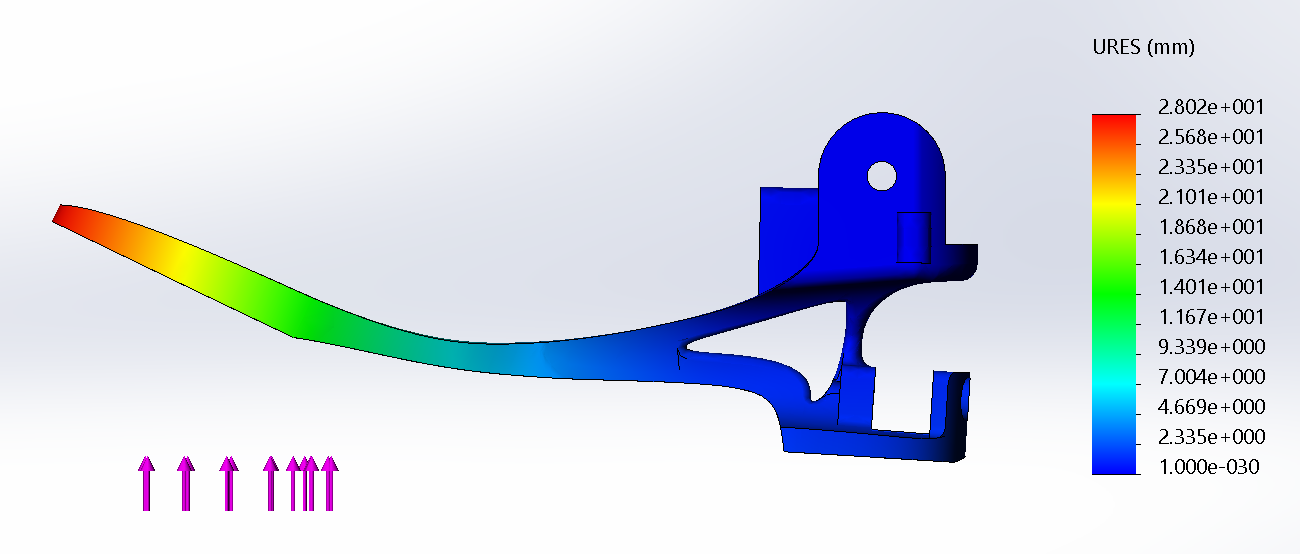
\includegraphics[width=\textwidth]{figures/fem_5N_1.PNG}
        \caption{FEM analysis in left foot iteration 1}
        \label{fig:fem_foot_iteration_1}
    \end{subfigure}
    \begin{subfigure}[b]{0.49\textwidth}
        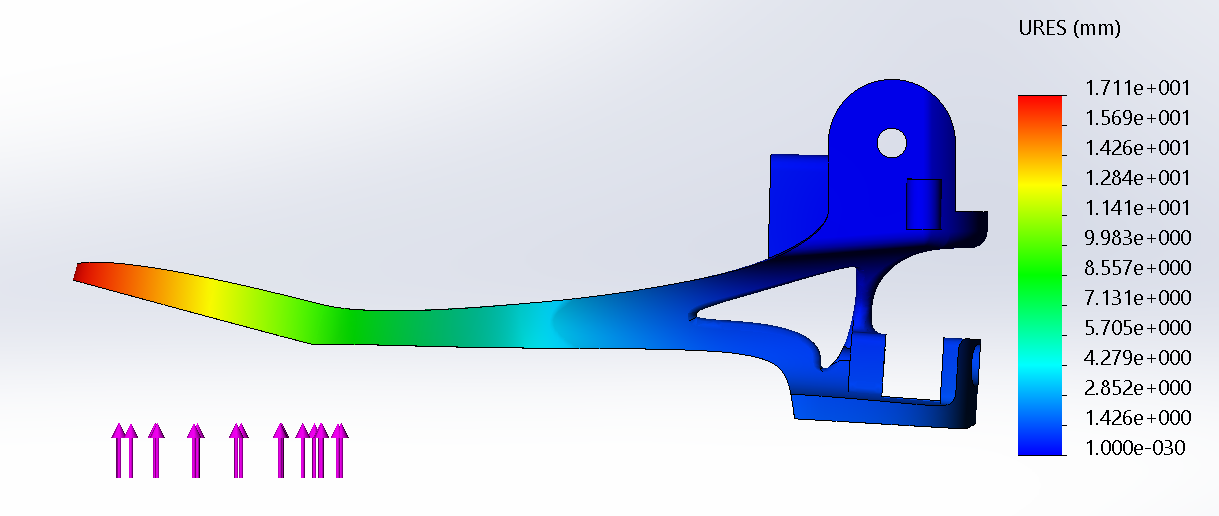
\includegraphics[width=\textwidth]{figures/fem_5N_2.PNG}
        \caption{FEM analysis in left foot iteration 2}
        \label{fig:fem_foot_iteration_2}
    \end{subfigure}
\end{figure}

% subsection finite_element_method (end)